\chapter{Correlators and Event-Table Data Analysis}
\label{chap:e14}

\begin{chapteropening}
In the previous chapter (Chapter~\ref{chap:e13}), the telescope wrote every photon candidate as one line of record: when it arrived, from which station, through which detector channel, at what wavelength, in what polarization. Over a single night, such records may number in the billions of lines; they lie quietly on disk, being in themselves neither an angular diameter nor a $g^{(2)}$, just a heap of time stamps.

What this chapter answers is precisely the process that lies between "a heap of events" and "a trustworthy curve": how do you turn these billions of time stamps into a $|V|^2$ or $g^{(2)}$ with error bars, one that is reproducible and can be taken away to fit physical models? We will follow one main thread: first translate the event table into a probabilistic model (write the likelihood), then define the correlation estimator and normalize it, then solve "can it be computed in finite time" (the computational scaling of the correlator), and finally the most underestimated link in all of the book's data analysis: where the errors come from, and why systematic error is so often the ceiling. The delay histogram given in Chapter~\ref{chap:e08}, and the Fisher-information language given in Chapter~\ref{chap:e12}, will here be genuinely put to use.
\end{chapteropening}

\section{From the event table to a probabilistic model}
\label{sec:e14-model}

Let us first agree on notation. Denote a calibrated event table as a whole by a dataset
\begin{equation}
  \mathcal{D}
  =
  \left\{
  t_q,\ a_q,\ d_q,\ c_q,\ p_q,\ w_q,\ f_q
  \right\}_{q=1}^{N_{\rm evt}} ,
  \label{eq:e14-data}
\end{equation}
\begin{formulaexplain}
$\mathcal D$ is the entire calibrated event table; each event $q$ carries a time $t_q$, station $a_q$, detector $d_q$, spectral channel $c_q$, polarization $p_q$, weight $w_q$, and quality flag $f_q$; $N_{\rm evt}$ is the total number of events. It is the raw "ingredient" of every estimator that follows.
\end{formulaexplain}
Here $t_q$ is the arrival moment on a unified time scale (units of s, with typical precision reaching nanoseconds or even tens of picoseconds), $a_q,d_q,c_q,p_q$ are all integer channel numbers (dimensionless), $w_q$ is the weight (dimensionless), and $f_q$ is the quality bit flagging whether this event is "clean." How these fields arise, how the clock is calibrated, and how the format is defined were the content of the previous chapter (Chapter~\ref{chap:e13}); this chapter starts directly from "the table already in hand."

The first step of the analysis is not to draw a plot, but to write down a \textbf{selection function}, which decides which events participate in the subsequent computation:
\begin{equation}
  S_q = S(t_q,a_q,d_q,c_q,p_q,f_q),
  \qquad
  S_q\in\{0,1\}\ \text{or}\ [0,1] .
  \label{eq:e14-selection}
\end{equation}
\begin{formulaexplain}
$S_q$ is the selection/weight of the $q$-th event; taking 0 or 1 means rejection or retention, while taking a continuous value in $[0,1]$ means a weighting due to exposure, dead time, background, or efficiency. It turns "manual point selection" into a rule that can be rerun.
\end{formulaexplain}
Why be so formal? Imagine a channel event rate of $10^{6}\,\mathrm{s^{-1}}$: a one-hour observation is $3.6\times10^{9}$ events. No one can "watch the plot and manually delete a few bad points", that is neither feasible nor reproducible. The selection function must be automatically regenerable from metadata (cloud cover, PMT current, dead-time flags, thresholds), so that the light-curve, correlation, and fitting layers all use the same criteria. When Chapter~\ref{chap:e15} does the error budget it will repeatedly emphasize: all systematic tests must be performed under the same set of $S_q$.

\paragraph{Unbinned data: the inhomogeneous Poisson point process}

Events are discrete points on the time axis, and the most natural model is the \textbf{inhomogeneous Poisson point process}: the instantaneous event rate at a given moment and channel is $\lambda(t,\bm{x}\mid\bm{\theta})$, where $\bm x$ packages the labels of channel, wavelength, polarization, sky position, etc., and $\bm\theta$ are the physical parameters we ultimately want to estimate. Chapter~\ref{chap:e03} explained: in a Poisson process, the probability of "one event occurring in a very short stretch of time" is proportional to the rate times the duration, and the stretches are mutually independent. We use exactly this to build up the likelihood step by step.

Cut the whole observation into many extremely narrow cells $\Delta t$, so narrow that each cell contains at most one event. The probability that the $i$-th cell "has one event" is about $\lambda_i E_i\,\Delta t$ ($E_i$ is the effective exposure of this cell), and the probability of "no event" is about $1-\lambda_i E_i\,\Delta t\approx e^{-\lambda_i E_i\Delta t}$. The likelihood of the whole observation is the product over all cells: occupied cells contribute $\lambda E\Delta t$, and empty cells contribute $e^{-\lambda E\Delta t}$. Take the logarithm:
\[
  \ln L
  =\sum_{q:\,S_q>0}\ln\!\big(\lambda(t_q,\bm x_q)\,E_q\,\Delta t\big)
   -\sum_{\text{all cells}}\lambda_i E_i\,\Delta t .
\]
Let $\Delta t\to0$: in the first term, $\ln\!\big(\lambda E_q\,\Delta t\big)=\ln\lambda+\ln E_q+\ln\Delta t$ can be split, where $\ln\Delta t$ is the binning width and $\ln E_q$ is the instrument/exposure term of this cell, both independent of the parameters $\bm\theta$ to be estimated and thus dropped together as constants in the fit (note that the exposure $E$ itself does not vanish; it is fully retained in the integral of the second term), so the first term keeps only $\ln\lambda$; the second sum becomes an integral. Hence
\begin{equation}
  \ln L(\bm\theta)
  =
  \sum_{q:\,S_q>0}\ln\lambda(t_q,\bm x_q\mid\bm\theta)
  -\int_{\mathcal T}\lambda(t,\bm x\mid\bm\theta)\,E(t,\bm x)\,dt\,d\bm x .
  \label{eq:e14-point-likelihood}
\end{equation}
\begin{formulaexplain}
$\ln L$ is the point-process log-likelihood. The first term scores the model rate at each real event: an event landing in a high-rate region gains points. The second term is the total number of events the model predicts over the effective exposure $E$: the model cannot merely spike at the events, it must also explain why there are no events elsewhere.
\end{formulaexplain}
Let us spell out each symbol: $\lambda$ has units of $\mathrm{s^{-1}}$ (or $\mathrm{s^{-1}\,channel^{-1}}$), $E(t,\bm x)$ is dimensionless or carries an area/efficiency factor, holding the real losses of bad weather, dead time, channel on/off, filter transmission, and observation window. The most important teaching point of this formula is its "balance": making the rate high only at the events cannot fool the second term, because the second term deducts points for predicting too many events. This is precisely the Cash statistic in astronomy, and at low counts one cannot get away with the symmetric $\sqrt N$ error \citep{1979ApJ...228..939C,1986ApJ...303..336G}.

\begin{figure}[tbp]
\centering
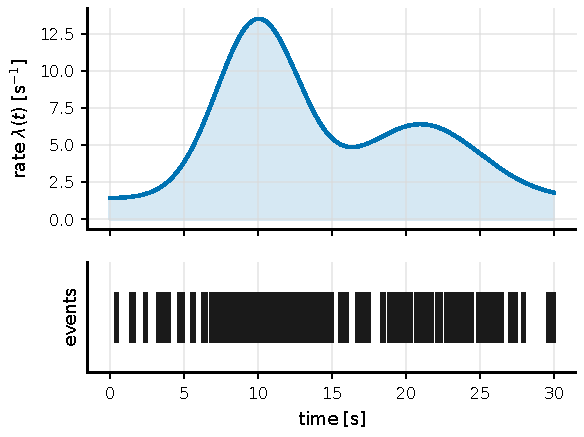
\includegraphics[width=0.72\linewidth]{figures/generated/chapter_07/ch07_poisson_likelihood.pdf}
\caption{The picture of an inhomogeneous Poisson process. The upper panel is the instantaneous rate $\lambda(t)$ fluctuating with time, and the lower panel is a string of events randomly "dropped" by this rate. The likelihood~\eqref{eq:e14-point-likelihood} uses both "events landing at high rate" and "the integrated rate over the whole stretch"; if the events are merely re-binned into a light curve, part of the time information is lost, especially for rapid variability or uneven exposure.}
\label{fig:e14-poisson}
\end{figure}

\paragraph{Binned data: degenerating to per-cell Poisson}

If we first bin the events into time cells, spectral channels, or delay cells, the point-process likelihood degenerates into the \textbf{binned Poisson likelihood} that everyone knows. The $i$-th cell observes $d_i$ events, the model predicts $m_i(\bm\theta)$, and the Poisson probability is $P(d_i)=e^{-m_i}m_i^{d_i}/d_i!$ (see Chapter~\ref{chap:e03}). The cells are independent; take the logarithm and sum:
\begin{equation}
  \ln L
  =\sum_i\Big[\,d_i\ln m_i(\bm\theta)-m_i(\bm\theta)-\ln(d_i!)\,\Big] .
  \label{eq:e14-binned-poisson}
\end{equation}
\begin{formulaexplain}
$d_i$ is the observed count of the $i$-th cell, $m_i$ the model count, both dimensionless. This is the likelihood usable by light curves, spectral channels, and delay histograms alike; it innately preserves the asymmetric statistics at low counts and does not pretend the errors are Gaussian.
\end{formulaexplain}
When a cell's count $d_i\gtrsim20$ and the model is not near a boundary, the Poisson can be approximated as Gaussian with error bars of about $\sqrt{d_i}$; but when a cell has only a few counts (as the signal window of a delay histogram often does), one must stay with Eq.~\eqref{eq:e14-binned-poisson}. There is another pitfall to mention in advance: when the model adds a component "whose strength must be nonnegative" (for example, "is there a correlation peak or not"), zero strength falls on the parameter boundary, the likelihood-ratio test no longer follows the nominal $\chi^2$ distribution, and the significance must be calibrated by simulation or posterior predictive checks \citep{2002ApJ...571..545P}. For slowly varying backgrounds and burst screening, Bayesian Blocks adaptively cuts the time axis into several "constant-rate segments," with data gaps entering through the effective exposure (live time) rather than being mistaken for "no events" \citep{2013ApJ...764..167S}; but the final physical parameters should still return to an explicit likelihood.

\section{How two streams of events grow a correlation peak}
\label{sec:e14-corr}

The core action of intensity interferometry is to compare the event arrival times of two stations $a,b$. Chapter~\ref{chap:e08} already obtained the idea of the delay histogram from $g^{(2)}$; here we cast it into an estimator that can run on real event tables.

The first step is to compute the \textbf{corrected time difference}. The raw time difference is mixed with the geometric delay and the instrument delay, which must be subtracted first:
\begin{equation}
  \tau_{ij}^{ab}
  =
  t_{j,b}^{\rm cal}-t_{i,a}^{\rm cal}
  -\Delta t_{\rm geo}^{ab}(t_i,\hat{\bm s})
  -\Delta t_{\rm inst}^{ab}(t_i) .
  \label{eq:e14-delay}
\end{equation}
\begin{formulaexplain}
$\tau_{ij}^{ab}$ is the corrected delay of two events at stations $a,b$; $t^{\rm cal}$ is the calibrated time, $\Delta t_{\rm geo}$ subtracts the geometric delay (the wavefront reaches the near telescope first), and $\Delta t_{\rm inst}$ subtracts the residual instrument delay of the two paths. It decides which delay cell this pair of events falls into.
\end{formulaexplain}
Why can the geometric delay not be neglected? For a 100 m baseline, the maximum time difference of the wavefront reaching the two telescopes is about $100/c\approx333\,\mathrm{ns}$; for a 1 km baseline it is $3.3\,\mu\mathrm{s}$. If the delay cell width is $\Delta\tau=4\,\mathrm{ns}$, then a geometric delay wrong by even one cell pushes the correlation peak away from zero delay and it vanishes outright. Furthermore, Earth is rotating, the projected baseline direction $\hat{\bm s}$ changes with time, and at tens-of-picoseconds precision the geometric delay must be continuously updated within very short time blocks \citep{2006MNRAS.369..655H,2006MNRAS.372.1549E,2018RNAAS...2....4K,2020NatAs...4.1164A}.

The second step is to count pairs: count all event pairs whose delay falls within the $k$-th cell $\tau_k\pm\Delta\tau/2$:
\begin{equation}
  C_{ab,k}
  =\sum_{i\in a}\sum_{j\in b}
  S_iS_j\,
  \mathbf 1\!\left[\tau_k-\tfrac{\Delta\tau}{2}\le\tau_{ij}^{ab}<\tau_k+\tfrac{\Delta\tau}{2}\right] .
  \label{eq:e14-paircount}
\end{equation}
\begin{formulaexplain}
$C_{ab,k}$ is the number of event pairs in the $k$-th delay cell; $S_iS_j$ weights each pair, and the indicator function $\mathbf 1[\cdot]$ picks only the pairs whose delay falls within that cell. It is one bar of the delay histogram, dimensionless.
\end{formulaexplain}

\paragraph{Normalization: the correlation peak is a faint excess on a background}

How tall one bar is has no meaning in itself, because even if the two streams were completely unrelated, pure randomness would still throw up a heap of "accidental coincidences." Assume the two streams are independent and their rates are approximately steady over the live time; the expectation of accidental coincidences can be estimated thus: stream $a$ has $R_aT_{\rm live}$ events in total, and each event has a probability of about $R_b\Delta\tau$ of "hitting" a stream-$b$ event within the delay cell $\Delta\tau$, and multiplying the two:
\begin{equation}
  B_{ab,k}\simeq R_aR_b\,\Delta\tau\,T_{\rm live} .
  \label{eq:e14-accidental}
\end{equation}
\begin{formulaexplain}
$B_{ab,k}$ is the accidental-coincidence background; $R_a,R_b$ (units $\mathrm{s^{-1}}$) are the two streams' mean rates, $\Delta\tau$ is the cell width, and $T_{\rm live}$ is the integration time after subtracting bad time. It is the number of accidental pairs that each cell should have "in the absence of celestial correlation."
\end{formulaexplain}
Plug in real numbers to feel the magnitude: take $R_a=R_b=10^{7}\,\mathrm{s^{-1}}$, $\Delta\tau=1\,\mathrm{ns}$, $T_{\rm live}=3600\,\mathrm{s}$, giving $B\approx10^{7}\times10^{7}\times10^{-9}\times3600\approx3.6\times10^{8}$. The background is as high as hundreds of millions of pairs, and the celestial correlation is only a tiny excess of order $10^{-6}$--$10^{-4}$ on top of it \citep{1974iiia.book.....H,2020NatAs...4.1164A,2024MNRAS.529.4387A}. Putting the two numbers together makes it clear: the signal $\approx3.6\times10^{8}\times10^{-4}\approx3.6\times10^{4}$ pairs, while the Poisson fluctuation of the background $\approx\sqrt{B}\approx1.9\times10^{4}$: after an hour the signal-to-noise ratio is only $\sim2$. Why intensity interferometry must integrate for tens of hours is written right here.

Dividing the bar by the background gives the normalized second-order correlation estimator and its excess:
\begin{equation}
  \widehat g^{(2)}_{ab}(\tau_k)=\frac{C_{ab,k}}{B_{ab,k}},
  \qquad
  \widehat C_{ab}(\tau_k)=\widehat g^{(2)}_{ab}(\tau_k)-1 .
  \label{eq:e14-g2}
\end{equation}
\begin{formulaexplain}
$\widehat g^{(2)}$ is the normalized second-order correlation, and $\widehat C_{ab}$ is the excess relative to the random background (dimensionless). The intensity-interferometry signal is hidden in this tiny excess after subtracting 1.
\end{formulaexplain}
In practice one rarely uses the analytic background of Eq.~\eqref{eq:e14-accidental} directly, but estimates $B$ using a \textbf{time-shift background}: shift stream $b$ as a whole by $\Delta T_{\rm shift}$, the shift being far larger than the correlation-peak width (so the true signal is moved away) yet far smaller than the slow-variation time of gain and rate (so the background structure is preserved). Averaging over multiple positive and negative shifts simultaneously gives the background mean and the background uncertainty. In addition there are stand-ins such as off-source (estimating skyglow, dark current), off-band (spectral-line science), and wrong-polarization (searching for crosstalk). VERITAS-SII rejects high-frequency electronic noise and low-PMT-current frames on 1-second correlation frames, then weights and averages the frames after the geometric-delay correction; MAGIC-SII uses the DC readings of the signal pixel and background pixel together to correct for night-sky light \citep{2020NatAs...4.1164A,2024MNRAS.529.4387A}.

\begin{figure}[tbp]
\centering
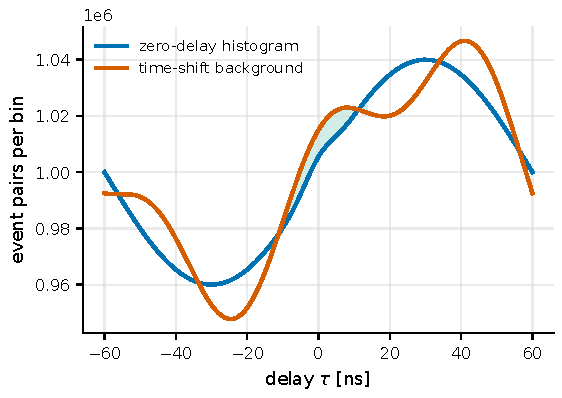
\includegraphics[width=0.72\linewidth]{figures/generated/chapter_07/ch07_time_shift_background.pdf}
\caption{The structure of time-shift background estimation. The blue curve is the event-pair histogram near zero delay, the orange curve is the accidental-coincidence background obtained by shifting one stream as a whole to a nonphysical delay, and the green region is the excess of the central peak relative to the time-shift background. This method preserves the slowly varying rate, bad time, and background structure, but the shift must be far larger than the instrument response width and the celestial correlation width.}
\label{fig:e14-timeshift}
\end{figure}

\paragraph{The continuous-waveform version: Pearson correlation}

If the hardware gives not discrete events but a continuously sampled voltage/current waveform (as MAGIC-SII does), the basic quantity becomes the \textbf{Pearson correlation coefficient}:
\begin{equation}
  \rho_{ab}(\tau_k)
  =\frac{\sum_n\big[x_a(t_n)-\bar x_a\big]\big[x_b(t_n+\tau_k)-\bar x_b\big]}
        {\sqrt{\sum_n\big[x_a(t_n)-\bar x_a\big]^2\;\sum_n\big[x_b(t_n)-\bar x_b\big]^2}} .
  \label{eq:e14-pearson}
\end{equation}
\begin{formulaexplain}
$\rho_{ab}$ measures the synchronous fluctuation of the two demeaned waveforms; $x_a,x_b$ are the sampled voltages/currents, and $\bar x$ is each one's mean. The denominator normalizes so that $\rho\in[-1,1]$; but it still mixes star, night-sky light, and electronic noise, and needs further calibration to become $|V|^2$.
\end{formulaexplain}
The Pearson correlation is very convenient to compute in real time in hardware (just demean, multiply, accumulate), but what it measures is a mixture of three fluctuations, and it must be calibrated with the DC current, background pixels, and zero baseline to be converted into the physical squared visibility $|V|^2$ \citep{2024MNRAS.529.4387A}. One last engineering detail: the cell width $\Delta\tau$ must be chosen together with the correlation-peak width and the time-stamp quantization: too wide dilutes the peak height, too narrow makes adjacent cells strongly correlated and inflates the computation for nothing; VERITAS-SII takes a correlation lag interval of 4 ns with a peak width also of about 4 ns, whereas a TDC of tens of picoseconds can cut the cells much finer, provided the geometric delay, instrument response, and clock residual are of equal precision \citep{2020NatAs...4.1164A,2020RScI...91a3108W,2009A&A...508..531N}.

\section{How the correlator finishes computing within a single night}
\label{sec:e14-scaling}

Now we face a purely engineering problem: that double sum in Eq.~\eqref{eq:e14-paircount}, can it really be computed?

\textbf{The most naive pair-by-pair method.} The two streams have $N_a,N_b$ events, and a full comparison is $N_aN_b$ differences; for the autocorrelation of the same stream, it is $N(N-1)/2$ pairs. Take $N_a=N_b=10^{9}$; that is $10^{18}$ differences, even at a billion per second ($10^{9}\,\mathrm{s^{-1}}$, roughly the realistic single-core speed), it would take $10^{18}/10^{9}=10^{9}\,\mathrm s\approx30$ years. The pair-by-pair method is fit only for small-sample teaching checks.

\textbf{The sorted-window method.} The true correlation peak lies only within a very narrow delay window, and there is no need to compare event pairs separated by several seconds. Sort both streams by time and look for pairs only within a sliding window $|t_{j,b}-t_{i,a}|\le W$; the number of candidate pairs to check is about
\begin{equation}
  N_{\rm pair}^{\rm win}\simeq 2W\,R_b\,N_a .
  \label{eq:e14-window}
\end{equation}
\begin{formulaexplain}
$N_{\rm pair}^{\rm win}$ is the number of candidate pairs the window method must check; $W$ (units s) is the maximum delay-window half-width, $R_b$ is the second stream's rate, and $N_a$ is the first stream's event count. A finite window brings the complexity from $N^2$ back to nearly linear.
\end{formulaexplain}
Substitute $W=100\,\mathrm{ns}$, $R_b=10^{6}\,\mathrm{s^{-1}}$, $N_a=10^{9}$: the candidate pairs are about $2\times10^{-7}\times10^{6}\times10^{9}=2\times10^{8}$, a full ten orders of magnitude fewer than the full double loop, and a workstation can sweep through them in a few minutes. Moreover, the sorted-window method preserves every event's full labels (wavelength, polarization), making re-selection afterwards convenient.

\textbf{FFT correlation: the XF and FX arrangements.} If the events or waveforms have already been placed into uniform time cells, one can use the fast Fourier transform to turn the time-domain cross-correlation into a frequency-domain multiplication:
\begin{equation}
  c_{ab}[k]
  =\mathcal F^{-1}\!\Big[\mathcal F\{x_a[n]\}^{*}\,\mathcal F\{x_b[n]\}\Big]_k .
  \label{eq:e14-fft}
\end{equation}
\begin{formulaexplain}
$c_{ab}[k]$ is the discrete cross-correlation; $\mathcal F,\mathcal F^{-1}$ are the forward/inverse discrete Fourier transforms, and the asterisk is complex conjugation. It replaces cell-by-cell multiply-accumulate ($O(N_{\rm bin}^2)$) with a single frequency-domain multiplication ($O(N_{\rm bin}\log N_{\rm bin})$), $N_{\rm bin}$ being the number of uniform time cells (a separate symbol is introduced here; do not confuse it with the $M$ denoting the number of time-shift backgrounds in the later error budget).
\end{formulaexplain}
Here appear the two kinds of correlator division of labour familiar from radio arrays: the \textbf{XF} type first does the cross-correlation (correlate, obtaining the delay-domain $c_{ab}[k]$) and then Fourier-transforms into a spectrum; the \textbf{FX} type does the reverse, first doing one FFT (Fourier) per stream, then cross-multiplying the streams pairwise in each frequency channel. Why is FX preferred once there are many stations? Because the FFT is a "once per stream" cost, growing linearly with the number of telescopes $N_{\rm tel}$; whereas the pairwise-multiply step is $O(N_{\rm tel}^{2})$ in either arrangement and cannot be avoided. When there are few stations (today's intensity-interferometry arrays often have only 2--4, so the number of pairs $N(N-1)/2$ is small), the bottleneck is not the number of pairs at all, but the \textbf{number of time samples each pair must swallow}: this is the correlator's real heavy lifting.

\begin{figure}[tbp]
\centering
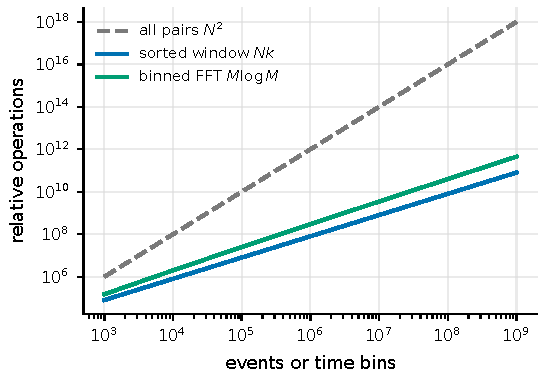
\includegraphics[width=0.72\linewidth]{figures/generated/chapter_07/ch07_correlator_scaling.pdf}
\caption{The operation-count scaling of three classes of correlation computation. The full pair-by-pair double loop grows wildly as $N^2$, suited only to small samples or teaching checks; the sorted window compares only pairs within a finite delay and is nearly linear; the FFT correlation after uniform binning grows as $N_{\rm bin}\log N_{\rm bin}$, suited to continuous sampling and real-time monitoring. The actual speed is further governed by memory bandwidth, I/O, GPU/FPGA data layout, and quality filtering.}
\label{fig:e14-scaling}
\end{figure}

\textbf{Real-time, dead-time-free hardware correlation.} VERITAS-SII streams the continuous PMT waveform to disk and then correlates offline with an FPGA; MAGIC-SII instead uses a GPU to compute all four-channel pairwise correlations in real time during the observation \citep{2020NatAs...4.1164A,2024MNRAS.529.4387A}. Continuous-waveform correlation has one advantage that single-photon counting cannot match: it does not rely on "trigger-and-reset per photon," and therefore has no dead-time blind spot of the kind a single-photon detector has after each count, and can compute the whole stretch of fluctuation into the correlation uninterruptedly; this is especially important for intensity interferometry with a signal of only $10^{-6}$--$10^{-4}$, where any time thrown away is signal-to-noise thrown away for nothing. Multi-channel TCSPC instead outputs a time-ordered event stream, convenient for constructing arbitrary delays and channel selections offline \citep{2020RScI...91a3108W}. Real-time correlation can also catch clock jumps, electronic crosstalk, and cloud-induced flux surges on the spot during observation, at the price of usually storing only the compressed correlation products. For long-term archiving, it is best to keep one copy each of the raw events/waveforms, calibrated events, and correlation products: FITS BINTABLE suits event archiving, HDF5/Parquet suits columnar big data, and Astropy helps handle FITS, time, and coordinate metadata \citep{2010A&A...524A..42P,2013A&A...558A..33A,2018AJ....156..123A}.

\section{Why the error is not a string of independent error bars}
\label{sec:e14-cov}

By now we have a $\widehat g^{(2)}(\tau_k)$ curve or a set of $|V|^2$. Fitting each point with a $\sqrt N$ error bar and treating them as mutually independent is the most common beginner's mistake. Let us first see how large the error should be in the ideal case, and then see why real data deviate from it.

Assume the signal-window count $C_{ab,k}$ is an independent Poisson quantity, the background is estimated by $M$ equal-weight time shifts, $\widehat B_{ab,k}=\frac1M\sum_{m=1}^{M}B_m$, and each $B_m$ is an independent Poisson quantity with mean $B$. How is the variance of the central excess $X=C-\widehat B$ computed? The variance of a Poisson quantity equals its mean, so $\operatorname{Var}(C)\approx C$; after averaging the background, $\operatorname{Var}(\widehat B)=\frac1{M^2}\sum_m\operatorname{Var}(B_m)=\frac1{M^2}\,(M\,B)=B/M$. The two are independent, and the variances add:
\begin{equation}
  \operatorname{Var}\!\big[\,C_{ab,k}-\widehat B_{ab,k}\,\big]
  \simeq C_{ab,k}+\frac{1}{M}\,B_{ab,k} .
  \label{eq:e14-excess-var}
\end{equation}
\begin{formulaexplain}
The first term $C_{ab,k}$ is the Poisson noise of the signal window itself, and the second term $B_{ab,k}/M$ is the residual uncertainty after averaging $M$ time-shift backgrounds. The larger $M$, the more stably the background is estimated. This is the error budget under the ideal of "independent events, steady rate."
\end{formulaexplain}
But Eq.~\eqref{eq:e14-excess-var} holds only when events are independent, time-shift backgrounds are mutually non-overlapping, and the rate is steady. Real data are full of "sharing" everywhere: adjacent delay cells share the same batch of events; multiple baselines share the same telescope; multiple wavelength channels share the same weather and the same gain path; multiple model points share the same zero-baseline normalization. Anything that is shared makes the errors of different data points \textbf{correlated}: the error matrix is no longer diagonal.

So one must treat all correlation products as a vector and equip it with a covariance matrix:
\begin{equation}
  \bm d=\big(\widehat{|V|^2}_1,\ \widehat{|V|^2}_2,\ \ldots,\ \widehat{|V|^2}_{N_d}\big),
  \qquad
  \Sigma_{ij}=\big\langle(d_i-\mu_i)(d_j-\mu_j)\big\rangle .
  \label{eq:e14-cov}
\end{equation}
\begin{formulaexplain}
$\bm d$ is the correlation-product data vector, $d_i$ is the $i$-th $|V|^2$ point, and $\mu_i$ is its mean; $\Sigma_{ij}$ is the covariance matrix, whose diagonal is each point's variance and whose off-diagonal records the correlated error caused by "shared telescope/background/calibration."
\end{formulaexplain}
Where does $\Sigma$ come from? Four routes: analytic error propagation (like Eq.~\eqref{eq:e14-excess-var}), time-block bootstrap, jackknife (removing one telescope or one night at a time), and end-to-end injection simulation. The time-block bootstrap is the most practical: cut the whole night's data into many time blocks, the block length being longer than the correlation-peak width, the electronic-noise correlation time, and the short-term pointing/weather fluctuation (for night-level data one often takes 10 s to a few minutes), randomly resample these blocks with replacement, and recompute $|V|^2$; the scatter between blocks directly gives the covariance, and as a bonus tests whether the error converges with integration time as $T^{-1/2}$. MAGIC-SII lists the electronic bandwidth, optical bandwidth, DC readout gain, background subtraction, and residual electronic noise all as systematic terms, and estimates the systematic error of the angular diameter by swinging the $|V|^2$ data points toward extreme directions \citep{2024MNRAS.529.4387A}.

\begin{figure}[tbp]
\centering
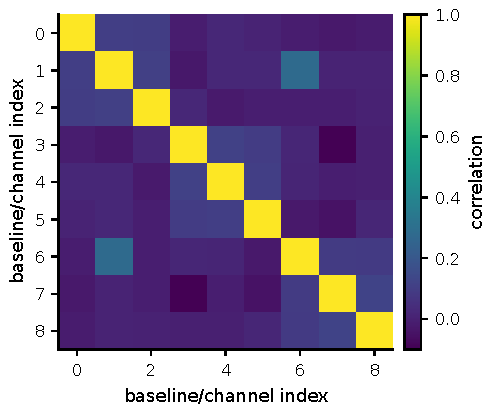
\includegraphics[width=0.66\linewidth]{figures/generated/chapter_07/ch07_covariance_matrix.pdf}
\caption{A schematic covariance matrix of multi-baseline/multi-channel results. The diagonal is the single-point variance, the blocks near the diagonal come from noise shared by the same time period or the same telescope, and the structure far from the diagonal may come from a common background estimate, zero-baseline normalization, or electronic crosstalk. If a fit uses only diagonal errors, it overestimates the "effective amount of independent information" and the error bars become spuriously small.}
\label{fig:e14-cov}
\end{figure}

One final piece of advice: all null tests must use the \textbf{same} selection function and weights as the main analysis. Common null tests include: shifting one stream to a nonphysical delay, swapping the sign of the geometric delay, using two polarization or wavelength channels that should not be correlated, using off-target sky as background, splitting the telescope pair into different time blocks, removing a certain telescope or night one at a time, and injecting a known correlation peak into the real event table to see whether it can be recovered without bias. If the main signal only appears below some threshold, and vanishes upon moving the threshold, using a wrong delay, or doing a jackknife, then it is more likely a product of pipeline selection or instrument state than a celestial correlation.

\section{White noise settles, systematic error is the ceiling}
\label{sec:e14-floor}

Chapter~\ref{chap:e12} used Fisher information to answer "how much information is really in the data." Here we connect it to time, and make clear the most critical watershed in an observation plan: white noise and systematic error have completely different fates.

\textbf{White noise (statistical noise) settles.} It comes from the Poisson fluctuation of photons and the random noise of electronics, one independent sample after another. The conclusion of Chapter~\ref{chap:e03}: the more independent samples, the more stable the mean, and the error falls with the effective photon number $N_{\rm eff}$ as $N_{\rm eff}^{-1/2}$, that is, with integration time as $T^{-1/2}$. In Fisher language, the information of independent data points \textbf{adds}, the total information grows linearly with $N_{\rm eff}$, and the parameter error given by the Cramér--Rao bound shrinks inversely as the square root of the information: as long as you are willing to integrate, it keeps falling.

\textbf{Systematic error (systematic bias) does not settle.} It comes from \textbf{consistent offsets} such as inaccurate calibration, imperfectly subtracted background, gain drift, a nonzero zero baseline, and biased electronic- or optical-bandwidth calibration. They are not independent samples each time, but push each data point the same little bit in the same direction. Integrate ten times longer and the white noise drops to $1/\sqrt{10}$, but this offset does not budge: it becomes a horizontal \textbf{floor}, and the error can go no lower.

Why is this floor especially deadly for us? Because the intensity-interferometry signal is inherently only as faint as $10^{-6}$--$10^{-4}$ (recall the example below Eq.~\eqref{eq:e14-accidental} of the $3.6\times10^4$-pair excess pressed on a $3.6\times10^8$ background). When the excess you want to measure is only one part in a million, then a consistent bias of just a few parts in a million in the background calibration is enough to be of the same order as the signal, or even to drown it. In other words: the faint signal presses the tolerance for systematic error down to the same demanding $10^{-6}$ level, and this is precisely the root of the field's dictum that "systematic terms are the ceiling."

To make this sentence mathematical, feed the covariance of Eq.~\eqref{eq:e14-cov} into the Fisher matrix (derivation in Chapter~\ref{chap:e12}):
\begin{equation}
  F_{\alpha\beta}
  =\frac{\partial\bm m^{T}}{\partial\theta_\alpha}\,\Sigma^{-1}\,\frac{\partial\bm m}{\partial\theta_\beta},
  \qquad
  \operatorname{Cov}(\theta_\alpha,\theta_\beta)\gtrsim(F^{-1})_{\alpha\beta} .
  \label{eq:e14-fisher}
\end{equation}
\begin{formulaexplain}
$F_{\alpha\beta}$ is the Fisher information matrix: $\partial\bm m/\partial\theta$ is the sensitivity of the model to the parameter, and $\Sigma^{-1}$ weights by the covariance. Its inverse $F^{-1}$ approximately gives the lower bound on the parameter covariance. It is the workhorse tool for observation planning and high-signal-to-noise error estimation.
\end{formulaexplain}
From this formula two scalings can be read at a glance. First, the \textbf{scaling with photon number}: if $\Sigma$ is dominated by independent photon statistics, then $\Sigma^{-1}\propto N_{\rm eff}$, $F\propto N_{\rm eff}$, and the parameter error $\propto N_{\rm eff}^{-1/2}$: this is the settling of white noise. Second, the \textbf{scaling with baseline}: the Fisher information is additive over mutually independent $uv$ points, $F=\sum_{\text{baselines}}$ (one term per baseline), so adding one more baseline adds one more piece of information. But whether a baseline is worth it depends on whether it falls where the model $|V|^2$ is most sensitive to the parameter, i.e. where $\partial\bm m/\partial\theta$ is largest: for measuring an angular diameter, the most valuable baseline falls near the first zero of the visibility curve (see the $uv$-coverage discussion of Chapters~\ref{chap:e10} and~\ref{chap:e11}), whereas a short baseline where $|V|^2\approx1$ carries almost no angular-diameter information. But once a systematic floor that does not fall with time appears in $\Sigma$, $\Sigma^{-1}$ saturates, and no matter how many more photons or how much longer the integration, $F$ no longer grows: the error tends to the floor and stops.

\begin{figure}[tbp]
\centering
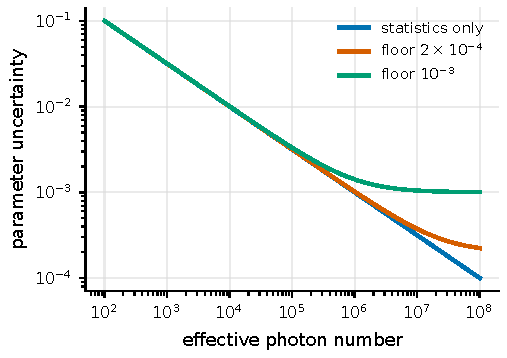
\includegraphics[width=0.70\linewidth]{figures/generated/chapter_07/ch07_fisher_scaling.pdf}
\caption{The scaling of parameter error with the effective photon number. The blue curve is the pure-statistical $N_{\rm eff}^{-1/2}$ settling; the orange and green curves, after adding systematic floors of different heights, no longer improve the final error at long integration. An observation plan must put integration time, target brightness, baseline coverage, and systematic calibration into the same error budget, which is precisely the theme of Chapter~\ref{chap:e15}.}
\label{fig:e14-fisher}
\end{figure}

A final reminder: the Fisher matrix is a local quadratic approximation near the likelihood peak, reliable only at high signal-to-noise and when the posterior is near-Gaussian. For a multi-peaked posterior, a nonlinear degeneracy, or a parameter near a boundary, one must switch to MCMC or nested sampling \citep{1925PCPS...22..700F,2013PASP..125..306F,2009MNRAS.398.1601F}.

\section{From correlation products to physical parameters}
\label{sec:e14-fit}

With the correlation products and their covariance in hand, the last step is to fit out the physical parameters. First write the \textbf{model vector}: map the angular diameter, binary separation, brightness ratio, ring radius, or jet parameters into the squared visibility at each $uv$ point and each wavelength:
\begin{equation}
  \bm m(\bm\theta)
  =\Big[\,|V(\bm u_1,\lambda_1\mid\bm\theta)|^2,\ \ldots,\ |V(\bm u_{N_d},\lambda_{N_d}\mid\bm\theta)|^2\,\Big] .
  \label{eq:e14-model}
\end{equation}
\begin{formulaexplain}
$\bm m(\bm\theta)$ is the data vector predicted by the physical model, each entry being the $|V|^2$ at spatial frequency $\bm u_i$ and wavelength $\lambda_i$. It translates the angular-diameter, binary, and structure parameters into observables directly comparable with $\bm d$.
\end{formulaexplain}
Here $\bm u=\bm B_\perp/\lambda$ is the spatial frequency (the projected baseline in units of wavelength, see the van Cittert--Zernike theorem of Chapter~\ref{chap:e10}). If the data vector $\bm d$ is already approximately Gaussian, the likelihood is the covariance-weighted residual:
\begin{equation}
  -2\ln L
  =\big[\bm d-\bm m(\bm\theta)\big]^{T}\Sigma^{-1}\big[\bm d-\bm m(\bm\theta)\big]
   +\ln|\Sigma|+\text{const} .
  \label{eq:e14-gauss}
\end{equation}
\begin{formulaexplain}
$\bm d-\bm m$ is the data-minus-model residual, $\Sigma^{-1}$ weights by the covariance (correlated points do not count information twice), and $\ln|\Sigma|$ is the normalization term. This is the most common Gaussian likelihood for data products with correlated errors, and minimizing it gives the optimal parameters.
\end{formulaexplain}
Note that the $\Sigma^{-1}$ step is precisely the payoff of Section~\ref{sec:e14-cov}: using the full covariance rather than diagonal errors is what prevents treating correlated points as mutually independent and overcounting the information. If you fit the raw low-count delay cells directly, do not use the Gaussian; return to the Poisson likelihood of Eq.~\eqref{eq:e14-binned-poisson}. VERITAS-SII fits the variation of $|g^{(1)}|^2$ with projected baseline using uniform-disk and limb-darkening models; MAGIC-SII converts the Pearson correlation into $|V|^2$ through flux and background calibration and then fits the angular diameter and systematic error \citep{2020NatAs...4.1164A,2024MNRAS.529.4387A,1967MNRAS.137..375H}.

When the posterior may be multi-peaked, or external priors are needed, write it as a \textbf{Bayesian posterior}:
\begin{equation}
  p(\bm\theta\mid\mathcal D,M)=\frac{L(\mathcal D\mid\bm\theta,M)\,\pi(\bm\theta\mid M)}{Z_M},
  \qquad
  Z_M=\int L\,\pi\,d\bm\theta .
  \label{eq:e14-posterior}
\end{equation}
\begin{formulaexplain}
$p(\bm\theta\mid\mathcal D,M)$ is the parameter posterior under model $M$, $L$ is the likelihood, $\pi$ is the prior, and $Z_M$ is the model evidence (the normalization constant, also used to compare models). It combines the data constraint and external physical knowledge into a complete uncertainty.
\end{formulaexplain}
The prior $\pi$ can hold the distance, spectral type, known angular diameter, binary orbit, burst time, or physical boundaries, and it must be stated clearly, because intensity interferometry often measures only $|V|^2$ and lacks the phase, causing mirror, brightness-ratio, and position-angle degeneracies, and it is the prior that helps hold the degeneracy down. As for sampling, emcee suits moderate-dimensional posteriors, and MultiNest suits multi-peaked posteriors and evidence estimation \citep{2013PASP..125..306F,2009MNRAS.398.1601F}; but the sampler cannot replace physical checks: the chain's autocorrelation time, acceptance rate, prior volume, and "whether an injected known signal can be recovered without bias" must all be reported together \citep{1992ApJ...398..146G}. Only then is the chain from event table to error-bearing parameters closed; Chapter~\ref{chap:e15} will put it into the complete observation design and feasibility assessment.

\section{Chapter Summary}
\label{sec:e14-summary}

\begin{itemize}
  \item \textbf{Build the model first, then compute the estimator.} The event table must first be written as a selection function Eq.~\eqref{eq:e14-selection} and a Poisson likelihood Eq.~\eqref{eq:e14-point-likelihood}/\eqref{eq:e14-binned-poisson}; the point-process likelihood arises naturally from "taking the limit of infinitely narrow bins," and preserves the time information lost after binning.
  \item \textbf{The correlation peak is a faint excess on a huge background.} The delay histogram Eq.~\eqref{eq:e14-paircount} only becomes meaningful after dividing by the accidental-coincidence background Eq.~\eqref{eq:e14-accidental}; the true signal is only $10^{-6}$--$10^{-4}$ of the background, which fundamentally determines the requirements on integration time and calibration precision.
  \item \textbf{Finishing the computation relies on algorithms, not brute force.} Pair-by-pair $N^2$/$N(N-1)/2$ is fit only for teaching; the sorted window Eq.~\eqref{eq:e14-window} is nearly linear, and the FFT (XF/FX) scales as $N_{\rm bin}\log N_{\rm bin}$; with few stations the bottleneck is the number of time samples each pair swallows, and GPU/FPGA real-time, dead-time-free correlation computes the whole stretch of fluctuation.
  \item \textbf{The error is not independent error bars.} Shared telescope, background, and calibration make off-diagonal terms appear in the covariance Eq.~\eqref{eq:e14-cov}; estimate $\Sigma$ with time-block bootstrap/jackknife/injection simulation, and the fit Eq.~\eqref{eq:e14-gauss} must use the full $\Sigma^{-1}$.
  \item \textbf{White noise settles, systematic error is the ceiling.} The statistical error falls with $N_{\rm eff}^{-1/2}$, $T^{-1/2}$, and the Fisher information grows linearly with photon number and adds over independent baselines; but a consistent offset forms a floor that does not fall with integration, and the faint signal presses the systematic tolerance down to the same demanding order.
\end{itemize}

\medskip
\noindent\textbf{Questions to Ponder.}
(1) If the delay cell width $\Delta\tau$ is halved, how do the accidental-coincidence background $B_{ab,k}$ and the signal excess each change, and does the final signal-to-noise ratio improve?
(2) You have 4 telescopes; why does "only 6 pairs" not mean the correlator is easy? On which quantity is the bottleneck?
(3) A team increased its integration time tenfold, but the error bars barely shrank. In this chapter's language, what is the most likely diagnosis? Which null tests should be done to confirm it?
